\chapter{Quickly Searching Explicit Expensive Graphs}
\label{chap:e8}

In order for an articulated robot to perform manipulation tasks
in changing, unstructured environments,
it must be able to quickly solve motion planning queries in its
configuration space.
In this chapter,
we discuss the efficiency tradeoffs induced by formulating
the articulated motion planning problem as best-first search,
propose a general planning framework which accounts for these tradeoffs,
and examine some empirical results.

\paragraph{Two Notions of Efficiency.}

Throughout this chapter,
we reference two different types of efficiency
with regard to robotic tasks.
First, once a planner has computed a solution path or trajectory,
there is the cost incurred while executing that trajectory.
This is the traditional cost optimized for by planners.
Second, there is the cost incurred from actually computing the solution
itself.

This dichotomy of effort is, of course, not new.
From Winston's \emph{Articifial Intelligence} \cite{winston1977ai},
\begin{quote}
   ``Properly speaking, the problem of determining a good path is a search
   problem in which two kinds of effort are involved:
   \begin{itemize}
   \item First, there is the effort expended in \emph{finding} either
      some path or the best path.
   \item And, second, there is the effort actually expended in
      \emph{traversing} the network.''
   \end{itemize}
\end{quote}

For the application of manipulation planning for articulated robots,
in paricular,
the costs associated with these two components tend to be of comparable
magnitude.
For example,
when time is used as an efficency metric,
both planning and execution times for household applications
tend to be on the order of 1-2 seconds.
Alternatively, given
modern computational and actuator technologies for human-scale problems,
both planning and execution tend to consume similar amounts of energy.
Therefore,
the manipulation problem demands that
(a) the cost of plans and
(b) the cost of planning both be considered.

\section{Explicit Graphs with Expensive Edge Evaluations.}

We have a graph $G$ with vertices $V$ and edges $E$.
We have some start set $V_s$ and some goal set $V_g$.
We represent a path through the graph as
$\pi = \{ v_0, v_1, v_2, \dots, v_n \}$;
a candidate solution path then has $v_0 \in V_s$ and $v_n \in V_g$.
We assume that only edges have costs,
such that the cost of a path is the cost if its constituent edges.
The cost of an edge is given by $x(v_a,v_b)$, and is always non-negative.
This requires that the execution cost functional be additive.
We assume that the graph is endowed with an admissible heuristic edge cost
function
$\hat{x}(v_a,v_b)$
which is inexpensive to compute.

We observe that such graphs motion planning for articulated robots
exhibit several properties that influence solution techniques.
See Figure~\ref{fig:seg-intro} for an example.

\paragraph{Small Graph Sizes.}
The size of a graph necessary to solve common problems
is relatively small.
In particular, it is reasonable to store the entire graph
\emph{explicitly} in memory;
techniques to incrementally build the graph
via an implicit graph representation
are not necessary.
Also,
we are not restricted to only expanding successors of a vertex;
we can simply make queries of the graph.

\paragraph{Expensive Edge Evaluations.}
Evaluating edge costs (e.g. testing for membership in
$\mathcal{C}_{\mbox{\scriptsize free}}$)
is expensive.
Planning times are dominated by edge evaluations
(as opposed to traditional graph search efficiency metrics
such as vertex expansions or heap percolates).

Another way of saying this is that in such a graph,
precious computation time is manifested in
\emph{evaluated edge costs},
not \emph{determined vertex $g$-values}.


\begin{figure}
   \centering
   \includegraphics{build/e8-exgraph-intro}
   \caption{A small explicit graph with some evaluated edges.}
   \label{fig:seg-intro}
\end{figure}

\section{Best-First Graph Search}
\label{sec:best-first}

In this section,
we discuss general best-first search over explicit graphs.

\subsection{Generic Best-First Search Algorithm over Paths}

Best-first search \cite{winston1977ai}
is a general class of search algorithms.
We choose to express the general algorith
over \emph{paths} instead of \emph{vertices}
for clarity and generality
because we are focused primarily on explicit graphs.
However, Section~\ref{sec:implicit} shows
how it reduces to traditional A* search
for certain types of evaluation functions,
as is required when searching over implicit graphs.

\begin{algorithm}
   \caption{Generic Best-First Search Algorithm Outline}
   \label{alg:generic-best-first}
   \begin{algorithmic}[1]
   \Procedure {\textsc{GenericBestFirst}}{$G$}
   \Loop
      \State $\pi^* = \argmin\limits_{\pi \in \Pi} f(\pi)$
         \Comment{For some path cost function $f(\pi)$}
         \label{line:generic-select-optimistic-path}
      \If {$\pi^*$ fully evaluated}
         \State \Return $\pi^*$
      \EndIf
      \State \textsc{EvalPath}$(\pi^*)$
         \Comment{For some evaluation function}
   \EndLoop
   \EndProcedure
   \end{algorithmic}
\end{algorithm}

Consider the general best-first search algorithm
(Algorithm~\ref{alg:generic-best-first}).
It maintains some sort of data structure storing known data about the
graph (e.g. tags on vertices or edges).
It simply iterates over optimistically-optimal ``best'' paths,
partially evaluating each.
(Note especially the greedy nature of this search.)
See Figure~\ref{fig:seg-edge-example} for a simple example.

\begin{figure}
   \centering
   \begin{subfigure}[b]{0.45\textwidth}
      \includegraphics{build/e8-exgraph-edge-select}
      \caption{Select optimistic best path}
   \end{subfigure}%
   \quad%
   \begin{subfigure}[b]{0.45\textwidth}
      \includegraphics{build/e8-exgraph-edge-eval}
      \caption{Evaluate first unevaluated edge}
   \end{subfigure}%
   \caption{Generic best-first algorithm for an explicit graph,
      with $f(\pi)$ best known cost-from-start,
      and {\sc Eval} forward edge evaluations.
      This algorithm is guaranteed to terminate with a feasible path
      with mimimum path cost, if one exists.}
   \label{fig:seg-edge-example}
\end{figure}

This formulation admits two choices:

\textbf{Cost Function $f(\pi)$.}
What is the cost function $f(\pi)$ over paths used to select the
path for evaluation at each iteration?
For now, we will use the following path objective:
\begin{equation}
   f(\pi) = \hat{f}_x(\pi): \mbox{\emph{optimistic estimate of execution effort}}.
\end{equation}
In other worts, $\hat{f}_x(\pi)$
gives a lower bound on the cost of executing
path $p$.
If the path consists of a mix of evaluated and unevaluated edges,
we could write this as:
\begin{equation}
   \hat{f}_x(\pi) = \sum_{e \in \pi} \left\{
   \begin{array}{cl}
      c[e] & \mbox{if edge } e \mbox{ evaluated}  \\
      \hat{c}(e) & \mbox{otherwise} \\
   \end{array}
   \right.
   .
   \label{eqn:execution-cost-objective}
\end{equation}

\textbf{Evaluation Procedure $\mbox{\sc EvalPath}(\pi)$}
How is a potential path evaluated?

The choice of these two components of the algorithm
intimately depend on the graph representation.
Note that we defer discussion of how the path minimization
(line~\ref{line:generic-select-optimistic-path}) until later,
and with it discussion of the algorithm's complexity.

\subsection{Best-First Search on Implicit Graphs}
\label{sec:implicit}

Figure~\ref{fig:seg-edge-example} searches an explicit graph,
in which the entire graph structure is represented in memory.
Here, we briefly discuss the application of
Algorithm~\ref{alg:generic-best-first}
to \emph{implicit} graphs,
and thereby relate this path-oriented treatment of graph search
to well-known existing algorithms.

Often, due to resource constraints or convenience,
the graph is instead expressed \emph{implicitly}
with one or more operators which calculate the structure of the graph
in the local vicinity of a given vertex.
Initialized with one or more vertices (e.g. starts and/or goals),
an algorithm can incrementally ``discover'' more of the
graph by repeatedly calling such function on discovered vertices.
As a result of this representation,
only a small portion of the graph might need to be explored
during the search.

Due to this implicit representation,
it is clear that each candidate path $\pi \in \Pi$ to be considered
(line \ref{line:generic-select-optimistic-path})
cannot generally exist of entirely known edges.
When enumerating candidate paths to the goal,
we must include potential ``virtual'' path segments
through the as-yet undiscovered portion of the graph
to approximate the path cost function $f(\pi)$.
The behavior of the search depends on this approximation,
as well as the nature of {\sc Evaluate} function induced by
the implicit representation operator(s) available.
Several variants are briefly discussed here.

\subsubsection{Relation to A*}

The most common implicit graph representation
is the \emph{expansion} or \emph{successor} function {\sc Successors}$(v)$
which yields all vertices reachable from the parent vertex $v$,
along with the associated edge costs.

Suppose, for now, that we only consider candidate paths that consist of:
(a) a first segment consisting over zero or more evaluated edges,
followed by
(b) an unexpanded ``frontier'' vertex $v_f$, followed by
(b) a second segment through the undiscovered portion of the graph.
We can then express $\hat{f}_x(\pi)$ as:
\begin{equation}
   \hat{f}_x(\pi)
   = \underbrace{f_{s \rightarrow v_f}(\pi)}_{g[v_f]}
   + \underbrace{f_{v_f \rightarrow g}(\pi)}_{h(v_f)}.
\end{equation}
These components correspond to the best-known cost-to-come $g[v_f]$
and the heuristic function $h(v_f)$ from A* search \cite{hart1968astar}.
See Figure~\ref{fig:seg-implicit} for an example with $h(v_f)=0$.

We can now produce a proof that as long as $h(v_f)$ is admissible,
and we are restricted to an {\sc Eval}$(\pi)$ function which 
expands the first unexpanded vertex,
the optimistic-optimal path $\pi^*$ at each iteration
follows the structure in the previous paragraph.
See Appendix~\ref{appendix:gs-proofs}.

\begin{figure}
   \centering
      \begin{subfigure}[b]{0.45\textwidth}
      \includegraphics{build/e8-exgraph-implicit-select}
      \caption{Select optimistic best path}
   \end{subfigure}%
   \quad%
   \begin{subfigure}[b]{0.45\textwidth}
      \includegraphics{build/e8-exgraph-implicit-expand}
      \caption{Expand first unexpanded vertex}
   \end{subfigure}%
   \caption{Best-first algorithm for an implicit graph,
      with $f(\pi)$ best known cost-from-start,
      and {\sc Eval} forward vertex expansions.
      This is Dijkstra's algorithm \cite{dijkstra1959anote}.}
   \label{fig:seg-implicit}
\end{figure}

Takeaway: A* uses a general heuristic function $h_g(v)$
because it doesn't have a representation of the full graph,
so it can't compute an actual best optimistic path.
I claim that for manipulation planning problems,
we can indeed reason over explicit graphs.

\subsubsection{Relation to BHFFA}

Let's say that we also have a function which computes the predecessors
of a vertex,
and also an admissible heuristic function $h(v_a,v_b)$ which computes
a lower-bound estimate of the optimal cost between two vertices.
Then the best-first thing to do is equivalent to the
Bidirectional Heuristic Front-to-Front Algorithm \cite{sint1977bhffa}.

\subsection{Best-First Search with Edge Evaluation}

What if, instead of operating over vertices (like A* and the like),
we operate over edges?
Figure~\ref{fig:seg-intro} illustrated the simplest such algorithm,
which selects the optimistic-optimal path,
and then evaluates the first as-yet unevaluated edge on the path.

Is the equivalent to regular A*
where the heuristic is the optimistic cost-to-goal?
(Only if all optimistic paths are all-evaled followed by non-evaled?)

I think that the forward-evaluation version of this is the same as
Optimal Generation A* (OPA*) and Simple Optimal Generation A* (SOGA*)
\cite{goldenberg2013epeastar},
which are modified versions of
Enhanced Partial Expansion A* \cite{felner2012epastar}.

\subsection{Bidirectional {\sc Eval} Procedures}

In general, over explicit graphs,
it usually makes sense to do bidirectional evaluations.
I need some data to back this up for my problem.
For example,
the Lazy PRM algorithm \cite{bohlin2000lazyprm}
is just best-first search
applied to binary edge cost functions
(that is, $x(e) \in \{ \hat{x}(e), \infty \}$)
with bidirectional edge evaluations
(although it actually uses a slightly fancier path evaluation function
-- see Chapter~\ref{chap:graphs-in-continuous}).

\section{Penalizing Planning Effort}

So far, we've been searching for a path which optimizes our solution
cost objective (\ref{eqn:execution-cost-objective}).
However, as we motivated in the introduction,
there are two distint notions of efficency,
and our objective so far (\ref{eqn:execution-cost-objective})
has only captured one of the two.
Here, we focus instead on \emph{planning efficiency},
and attempt to define an objective which captures it.
We hope that doing so will lead to searches which consume less 
time or energy.

\begin{equation}
   f(\pi) = \hat{f}_p(\pi) : \mbox{\emph{optimistic estimate of planning effort}}.
\end{equation}

What type of metric should we use?

\subsection{Metrics for Planning Effort}

For problems over very large graphs,
planning effort may be dominated by expanding vertices
or maintaining priority queues.
Therefore, traditional metrics for evaluating planning
effort are \emph{vertices expanded}
and \emph{heap percolates}.
However, for many manipulation problems,
search time is instead dominated by edge evaluations.

Therefore, we introduce a new objective $\hat{f}_p$
which penalizes remaining effort required to evaluate edges
along a potential path:
\begin{equation}
   \hat{f}_p(\pi) = \sum_{e \in \pi} \left\{
   \begin{array}{cl}
      0 & \mbox{if edge } e \mbox{ evaluated}  \\
      \hat{p}(e) & \mbox{otherwise} \\
   \end{array}
   \right.
   .
\end{equation}
This uses a new heuristic $\hat{p}(e)$ which estimates the cost
associated with evaluating an edge.
This could be planning time, computational energy required, etc.

The first graph planner to explicitly include such a heuristic
to estimate the remaining
computational planning effort in a best-first search
was A$_\epsilon^*$ \cite{pearl1982semiadmissible}.
While the approach we take is different from that of
\cite{pearl1982semiadmissible},
a motivating quote from this paper is relevant:
\begin{quote}
``The heuristic [\,$\hat{x}$\,] ... is of an entirely
different nature than the ... heuristic [\,$\hat{p}$\,] ... .
The former anticipates the reduction in \emph{solution quality} due to the
remaining part of the solution once it is found;
the latter estimates the \emph{computational effort}
required for completing the search.''
\end{quote}

Sidenote: RRT-Connect is sort of explicitly doing this
(optimizing at each step only for planning time,
but constrained to pass through the sampled point).

\subsection{Ensemble Effort Objective}

In general, we might consider weighting each objective:
\begin{equation}
   f(\pi) = \lambda \hat{f}_p(\pi) + (1 - \lambda) \hat{f}_x(\pi) .
   \label{eqn:general-objective}
\end{equation}
We call this effort model
\emph{ensemble effort}
in that it combines both planning and execution effort.
Note that with $\lambda=0$,
we recover our old solution cost objective $\hat{f}_x(\pi)$.
Note that this objective is used in an optimistic, greedy fashion at each
iteration of best-first search.
Represented over edges,
this can then be written:
\begin{equation}
   f(\pi) = \sum_{e \in \pi} \left\{
   \begin{array}{cl}
      (1 - \lambda) x[e] & \mbox{if edge } e \mbox{ evaluated}  \\
      \lambda \hat{p}(e) + (1 - \lambda) \hat{x}(e) & \mbox{otherwise} \\
   \end{array}
   \right.
   .
   \label{eqn:general-objective-explicit}
\end{equation}

We represent a particular choice of $\hat{p}(e)$
and $\hat{x}(e)$ as an \emph{ensemble effort model}
denoted with $\mathcal{M}$.
This is the objective used by the E$^8$ algorithm,
described in Section~\ref{sec:e8-planner}.

\subsection{Simplification with Propotional Heuristics}

Suppose that our edge evaluation cost heuristic
were proportional to our edge execution cost heuristic,
\begin{equation}
   \hat{p}(e) = \alpha \, \hat{x}(e) .
\end{equation}
This might happen if, for example, each were proportional to the edge's
\emph{distance} (with longer paths taking longer to both collision check
and execute at constant velocity).
In this case, we can write:
\begin{equation}
   f(\pi) = (1-\lambda) \sum_{e \in \pi} \left\{
   \begin{array}{cl}
      x[e] & \mbox{if edge } e \mbox{ evaluated}  \\
      \left[ 1 + \frac{\alpha\lambda}{1 - \lambda} \right] \hat{x}(e) & \mbox{otherwise} \\
   \end{array}
   \right.
   .
   \label{eqn:prop-heuristics}
\end{equation}

\subsection{Equivalence to Weighted A*}

Consider the case where we're using forward vertex or edge evaluations
(as is required with implicit graph representations),
and $\lambda < 1$.
In this case, we can rewrite (\ref{eqn:prop-heuristics})
simply as:
\begin{equation}
   f(\pi) \propto
   \underbrace{\sum_{e \; \mbox{\scriptsize evaled}} x[e]}_{g[v_f]}
   +
   \underbrace{\left[ 1 + \frac{\alpha \lambda}{1-\lambda} \right]}_{
      \mbox{\scriptsize inflation factor } \epsilon}
   \underbrace{\hat{x}(e_{last})}_{h(v_f)}
   .
\end{equation}

In other words,
\emph{weighted A* is equivalent to
   best-first search whose objective
   includes a planning effort term
   proportional to execution effot.}

In particular, if planning effort is proportional to execution
effort by a factor of $\alpha$,
a weighted A* search with inflation factor $\epsilon$
is the result of best-first search with
$\lambda = \frac{\epsilon-1}{\alpha+\epsilon-1}$.

\subsection{Relation to Experience Graphs}
\label{sec:egraphs}

Experience graphs \cite{phillips2012egraphs}
are a type of best-first search which
are designed to find paths quickly by incentivizing the planner
to rely on on edges from previous successful plans.

While the E-graph planner is originally expressed over implicit graphs,
we can instead express it as best-first search over paths
with the following objective:
\begin{equation}
   f_{\mbox{\scriptsize E-graphs}}(\pi) \propto \sum_{e \in \pi} \left\{
   \begin{array}{cl}
      x[e] & \mbox{if edge } e \mbox{ evaluated, this search} \\
      \epsilon \, x[e] & \mbox{if edge } e \mbox{ evaluated, previous search} \\
     \epsilon \, \epsilon^E \, \hat{x}(e) & \mbox{otherwise} \\
   \end{array}
   \right.
\end{equation}

The E$^8$ algorithm
is equivalent to the E-Graph algorithm
with $\epsilon=1$ and $\epsilon^E = 1 + \frac{\alpha \lambda}{1-\lambda}$.
We don't do E-graph shortcuts,
which are not necessary for small explicit graphs.
\cdnote{What about snap motions?}

\section{The E$^8$ Explicit Graph Search Algorithm}
\label{sec:e8-planner}

The E$^8$ algorithm
(Exploiting Ensemble Effort Estimates
on Explicit graphs with Expensive Edge Evaluations)
is the result of applying
best-first search with the $\lambda$-mediated objective
from (\ref{eqn:general-objective}).
Based on empirical results, we also use the bidirectional edge evaluation
algorithn,
since it tends to finish faster.

The E$^8$ algorithm is \emph{multi-query},
in that it maintains a data structure of evaluated edge
execution costs $x_{\mbox{\scriptsize eval}}[\cdot]$
which allows reuse between different planning problems
over the same graph $G$.

The algorithm is also \emph{lazy},
in that edge evaluations are deferred until they are needed.
In fact, it can be seen as a generalization of the
LazyPRM \cite{bohlin2000lazyprm}
which also considers planning effort in its objective.

Further,
the algorithm is \emph{heuristic-focused},
guided by its cost model $\mathcal{M}$.
Its behavior mimics that of an inflated heuristic planner
depending on the selection of the planning/execution cost
tradeoff parameter $\lambda$
as described in Section~\ref{subsec:choosing-lambda}.

\subsection{E$^8$ Algorithm Description}
\label{subsec:alg-e8-description}

\begin{algorithm}[t]
\caption{E$^8$ Explicit Graph Search}
\label{alg:e8}
\begin{algorithmic}[1]
   \Procedure {E$^8$}{$G,
      V_{\mbox{\scriptsize start}}, V_{\mbox{\scriptsize goal}},
      \mathcal{M}, \lambda$}
   \State $x_{\mbox{\scriptsize eval}}[\cdot] \leftarrow$ empty map
      ($x_{\mbox{\scriptsize eval}} : E \rightarrow \mathbb{R}_0^+$)
      \label{line:store-edge-eval-efforts}
   \ForAll {$e \in G$}
      \State $e.{\mbox{cost}} \leftarrow
         \lambda \, \hat{p}(e) + (1 - \lambda) \, \hat{x}(e)$
         \Comment Ensemble effort model $\mathcal{M}$
         \label{line:edge-cost}
   \EndFor
   \Loop
         \label{line:best-first-start}
      \State $\pi^* = \mbox{\sc BiDijkstras}(G,
         V_{\mbox{\scriptsize start}}, V_{\mbox{\scriptsize goal}})$
         \label{line:e8-select-optimistic-path}
      \If {$e \in x_{\mbox{\scriptsize eval}} \;\forall\; e \in \pi^*$}
         \State \Return $\pi^*$
            \label{line:return-done}
      \EndIf
      \State $E_{\mbox{\scriptsize to\_eval}} \leftarrow
         \mbox{\sc PathEvalOrder}(\pi^*)$
         \Comment{See Section \ref{subsec:alg-path-evaluation}}
         \label{line:path-eval-order}
      \ForAll {$e \in E_{\mbox{\scriptsize to\_eval}}$}
         \State $x_{\mbox{\scriptsize eval}}[e] \leftarrow x(e)$
            \Comment Evaluate edge (expensive!)
            \label{line:evaulate-edge}
         \State $e.{\mbox{cost}} \leftarrow
            (1 - \lambda) \, x_{\mbox{\scriptsize eval}}[e]$
            \Comment Update ensemble estimate
            \label{line:update-estimate}
         \If {$x_{\mbox{\scriptsize eval}}[e] > \hat{x}(e)$}
            \label{line:exec-cost-check}
            \State \textbf{break}
               \label{line:eval-break}
         \EndIf
      \EndFor
   \EndLoop
      \label{line:best-first-end}
   \EndProcedure
\end{algorithmic}
\end{algorithm}

The E$^8$ algorithm (Algorithm~\ref{alg:e8})
directly follows the outline
of best-first serach over paths
(Algorithm~\ref{alg:generic-best-first}).
Since edge evaluations are expensive,
we maintain a map $x_{\mbox{\scriptsize eval}}[\cdot]$
storing the known execution costs of all edges evaluated so far
(line~\ref{line:store-edge-eval-efforts}).
We also maintain a cost for each edge (line~\ref{line:edge-cost})
derived from the problem's ensemble effort model $\mathcal{M}$.

At each iteration,
we optimistically select the best path $\pi^*$
which minimizes the this ensemble objective.
We select over all paths which connect
a node in $V_{\mbox{\scriptsize start}}$
to a vertex in $V_{\mbox{\scriptsize goal}}$
(any-to-any);
for other types of planner specifications,
see Chapter~\ref{chap:cmr}.
We currently implement the algorithm's best-first search
using a bidirectional variant of
Dijkstra's algorithm \cite{dijkstra1959anote}
on line~\ref{line:e8-select-optimistic-path}.
See Section~\ref{subsec:search-each-iteration} below
for more details.

If this path is already fully evaluated,
we finish (line~\ref{line:return-done}).
Note that if edge costs $x(e)$ may be infinity
(e.g. to denote an infeasible edge),
the algorithm will terminate with a fully evaluated path
with infinite cost if no feasible path exists.

Otherwise,
we evaluate the path's unevaluated edges
(lines \ref{line:path-eval-order}
to \ref{line:eval-break}).
We do this in a particular order --
a discussion of possible orders follows in 
Section~\ref{subsec:alg-path-evaluation}.
For each edge,
we evaluate its execution cost $x(e)$ (line~\ref{line:evaulate-edge})
and update our effort estimate (line~\ref{line:update-estimate})
to account for (a) the actual execution effort
and (b) the fact that no additional planning effort is needed.
If the execution cost of any edge of the path proves
more expensive than we had anticipated
(line~\ref{line:exec-cost-check}),
we break and select a new path.

The E$^8$ algorithm admits a number of choices
which we discuss in the remainder of this section.

\subsection{Choosing $\lambda$}
\label{subsec:choosing-lambda}

The E$^8$ algorithm's objective,
from (\ref{eqn:general-objective-explicit}),
trades off between planning and execution effort,
mediated by the parameter $\lambda \in [0,1]$.
Loosely,
adjusting $\lambda$ varies the behavior between
\emph{feasibility} (finding paths quickly)
and \emph{optimality} (of execution).

With $\lambda=0$,
E$^8$ focuses solely on minimizing execution effort.
This is similar to the LazyPRM algorithm.
On the other hand,
with $\lambda=0$,
it focuses solely on minimizing planning effort,
similarly to the RRT algorithm.
We discuss these comparisons to existing continuous-space planners
in Chapter~\ref{chap:graphs-in-continuous}.

If our ensemble effort model $\mathcal{M}$
specifies effort estimates in the same units
(e.g. time or energy),
$\lambda=\frac{1}{2}$ is a natural choice.
However,
due to the optimistic nature of the E$^8$ algorithm,
a different value of $\lambda$ may perform better in practice.
See research question \ref{ques:choosing-lambda}
to a discussion about choosing this parameter.

\subsection{Finding the Optimistic-Optimal Path}
\label{subsec:search-each-iteration}

The current implementation of E$^8$ uses
bidirectional Dijkstra's algorithm
(line~\ref{line:e8-select-optimistic-path})
to select the lowest-cost path through the graph
at each iteration of the algorithm.
However, since the cost of only a few edges
are adjusted at each iteration (line~\ref{line:update-estimate}),
it appears that it is well-suited to incremental
graph search algorithms (e.g. \cite{koenig2004lpastar}).
See research question \ref{ques:incremental-search}
for discussion regarding improving the efficiency of this search.

\subsection{Path Edge Evaluation Order}
\label{subsec:alg-path-evaluation}

Once a candidate path is selected,
its constituent unevaluated edges are evaluted
in a particular order (line~\ref{line:edge-evaluation-order}).
Our current algorithm
orders the edges alternating from the ends in
(I need a figure to show this).
With different choices (e.g. forwards or backwards),
E$^8$ looks a lot like A$^*$.

\subsection{Repeated Queries}

Note that while
algorithm~\ref{alg:e8} supposes that you completely solve
one problem before moving on to the next,
the explicit graph representation
allows the E$^8$ algorithm
to natually extend to solving multiple problems,
either sequentially or interleaved.

For multiple queries within the same
$\mathcal{C}_{\mbox{\scriptsize free}}$,
the edge evaluations can be used in subsequent searches.
This ends up behaving similarily to E-graphs \cite{phillips2012egraphs}
with $\epsilon=1$
as described in Section~\ref{sec:egraphs},
with the exception that all evaluated edges are placed in the graph,
not just the edges on the solution path.

\section{Results}

\begin{figure}
   \centering
   % for stats
   \input{build/e8-world-astar-stats}
   \input{build/e8-world-wastar-stats}
   \input{build/e8-world-e8-stats}
   \begin{subfigure}[t]{0.47\textwidth}
      \centering
      \includegraphics{build/e8-world-intro}
      \caption{intro}
   \end{subfigure}%
   \quad%
   \begin{subfigure}[t]{0.47\textwidth}
      \centering
      \includegraphics{build/e8-world-astar}
      \caption{astar\\
         plan: \worldstatsastarplan\\
         exec: \worldstatsastarexec}
   \end{subfigure}%
   \quad%
   \begin{subfigure}[t]{0.47\textwidth}
      \centering
      \includegraphics{build/e8-world-wastar}
      \caption{wastar, $\epsilon=3$\\
         plan: \worldstatswastarplan\\
         exec: \worldstatswastarexec}
   \end{subfigure}%
   \quad%
   \begin{subfigure}[t]{0.47\textwidth}
      \centering
      \includegraphics{build/e8-world-e8}
      \caption{e8, $\lambda=0.5$\\
         plan: \worldstatseEplan\\
         exec: \worldstatseEexec}
   \end{subfigure}
   \caption{An E$^8$ example world problem.}
\end{figure}

Here are results.
See Figure~\ref{fig:bean} and Figure~\ref{fig:herb-comparison-cdfs}.

\begin{center}
\begin{tabular}{lrrr}
\toprule
Algorithm & Eval Effort & Vertex Expansions & Heap Percolates \\
\midrule
A$^*$ & 5 & 5 & 5 \\
Weighted A$^*$ & 5 & 5 & 5 \\
E-Graphs & 5 & 5 & 5 \\
E$^8$ & 5 & 5 & 5 \\
\bottomrule
\end{tabular}
\end{center}

I hope to show that the Greedy PRM is competitive with RRT-Connect
in terms of planning effort required to find a feasible path.

\begin{figure}
   \centering
   \begin{subfigure}[b]{0.3\textwidth}
      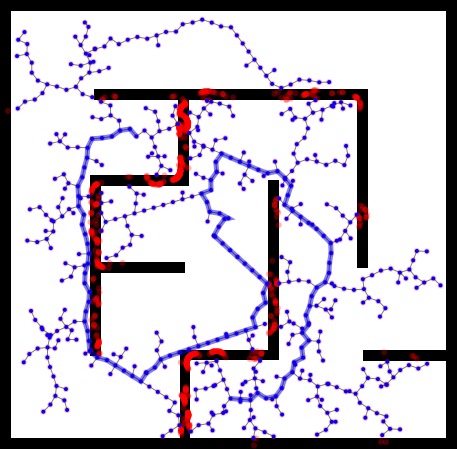
\includegraphics[width=\textwidth]{figs/compare-2d-rrtc1-rrtextcon-r1-s1.png}
      \caption{RRT Ext-Con, R=1}
   \end{subfigure}%
   \quad
   \begin{subfigure}[b]{0.3\textwidth}
      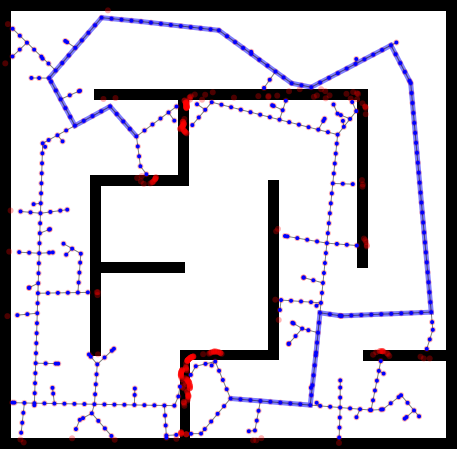
\includegraphics[width=\textwidth]{figs/compare-2d-rrtc1-rrtconcon-r1-s1.png}
      \caption{RRT Con-Con, R=1}
   \end{subfigure}%
   \quad
   \begin{subfigure}[b]{0.3\textwidth}
      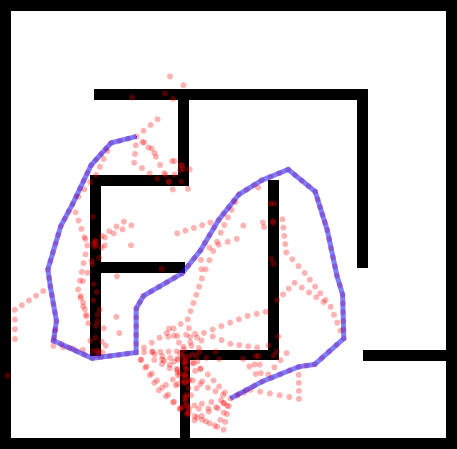
\includegraphics[width=\textwidth]{figs/compare-2d-rrtc1-checkmask-l00-s1.png}
      \caption{Greedy PRM, $\lambda=0$}
   \end{subfigure}%
   \vspace{0.05in}
   \begin{subfigure}[b]{0.3\textwidth}
      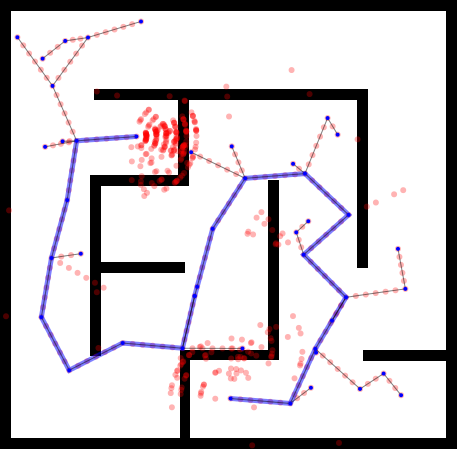
\includegraphics[width=\textwidth]{figs/compare-2d-rrtc1-rrtextcon-r6-s1.png}
      \caption{RRT Ext-Con, R=6}
   \end{subfigure}%
   \quad
   \begin{subfigure}[b]{0.3\textwidth}
      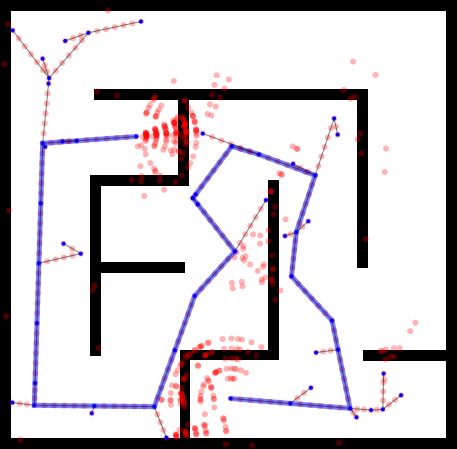
\includegraphics[width=\textwidth]{figs/compare-2d-rrtc1-rrtconcon-r6-s1.png}
      \caption{RRT Con-Con, R=6}
   \end{subfigure}%
   \quad
   \begin{subfigure}[b]{0.3\textwidth}
      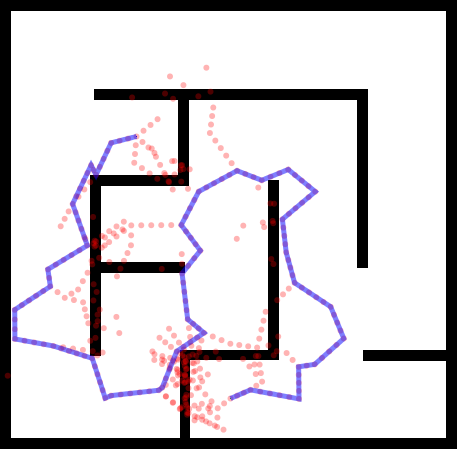
\includegraphics[width=\textwidth]{figs/compare-2d-rrtc1-checkmask-l10-s1.png}
      \caption{Greedy PRM, $\lambda=1$}
   \end{subfigure}%
   \caption{Example runs with different planners,
      with the same sequence of samples.
      Note that Greedy PRM $\lambda=0$ is equivalent to LazyPRM.
      Red dots show collision checks.}
   \label{fig:compare-2d-rrtc1-vis}
\end{figure}

\begin{figure}
\centering
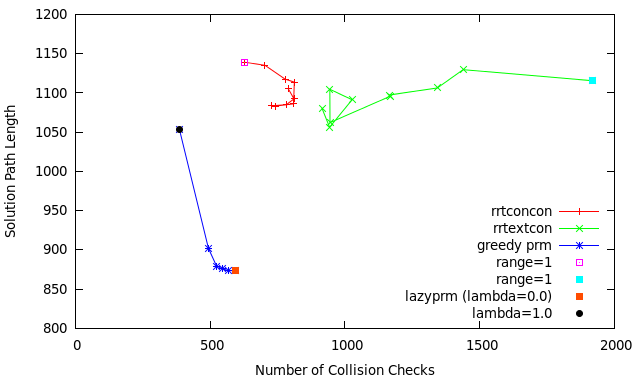
\includegraphics[width=0.8\textwidth]{figs/compare-2d-rrtc1-medians.png}
\caption{Plot of collision checks vs solution path cost for the
   different algorithms from the problem from
   Figure~\ref{fig:compare-2d-rrtc1-vis}.}
\end{figure}

\begin{figure}
   \centering
   \begin{subfigure}[b]{0.4\textwidth}
      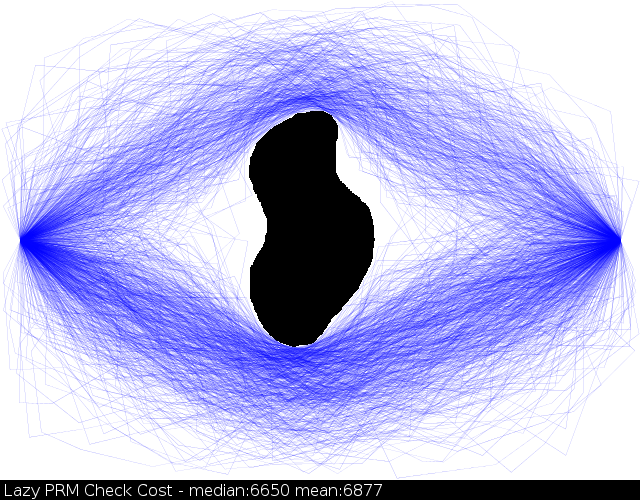
\includegraphics[width=\textwidth]{figs/timegreedy-bean-lambda-00.png}
      \caption{Paths with $\lambda = 0$}
   \end{subfigure}%
   \quad
   \begin{subfigure}[b]{0.4\textwidth}
      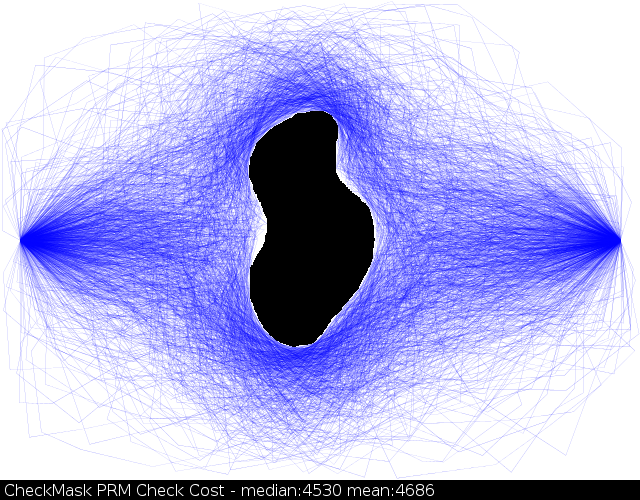
\includegraphics[width=\textwidth]{figs/timegreedy-bean-lambda-10.png}
      \caption{Paths with $\lambda = 1$}
   \end{subfigure}%
   \caption{Examples of paths for a 2d problems
      for different values of $\lambda$.
      As $\lambda$ is increased,
      paths are longer, but are faster to find.}
   \label{fig:bean}
\end{figure}

\begin{figure}
   \centering
   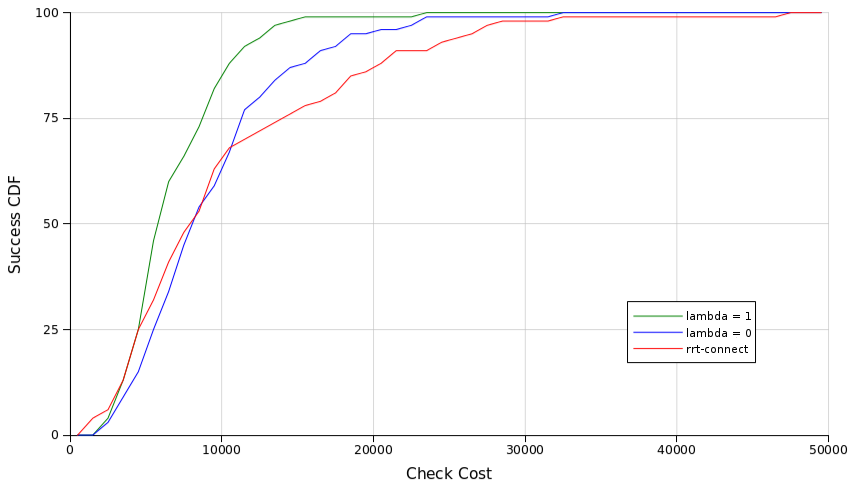
\includegraphics[width=0.8\textwidth]{figs/timegreedy-herbstep1-comparison-cdfs.png}
   \caption{Comparison between different algorithms on a HERB problem.
      Must add in ESTs.}
   \label{fig:herb-comparison-cdfs}
\end{figure}
